\chapter{Results} \label{cha:Results}
Now we have the fundamental background for the FEA. We begin this chapter by deriving physical meaning of the stiffness matrix. This is done for a simplified, but important version of \cref{prb:Non_Normalized_Problem}. Then apply FEM to some variations of \cref{prb:Non_Normalized_Problem}, namely \cref{cas:q_1st_Degree_Denom,cas:q_2nd_Degree_Denom,cas:q_Exponential}, see \cref{cha:Mechanical_Problem}. In each case we calculate the FEM-solution with both the linear and cubic basis-functions and for different No. of elements. To study FEM-convergence we will then compare these solutions with the known analytical solution.
%
\section{Derivation of Stiffness Matrix}
\begin{figure}
	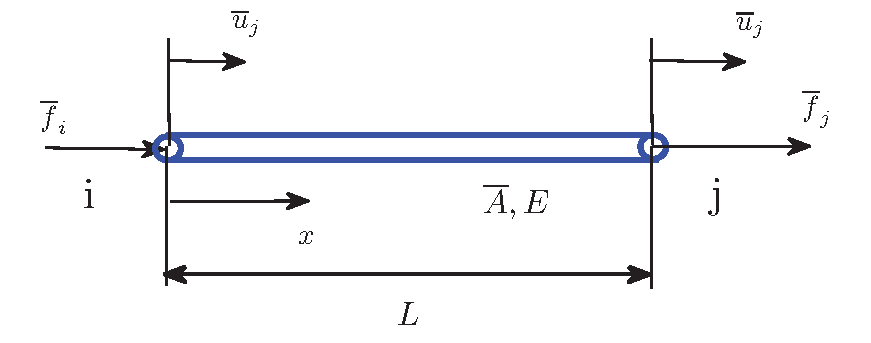
\includegraphics[width=\textwidth]{../figures/a-typical-element}
	\caption{A Typical Bar Element}
	\label{fig:A_Typical_Element}
\end{figure}
Imagine a uniform prismatic bar of length \gls{L}, cross-sectional area $\overline{A}$ and modulus of elasticity $E$. The bar is
elongated \gls{Delta} under an axial uniform force \gls{F}, see \cref{fig:A_Typical_Element}. This is obviously simplified version
of \cref{prb:Non_Normalized_Problem} as both \glssymbol{q} and \glssymbol{f} are constant. In this section we apply first FEM to
derive stiffens matrix for this problem. Then we look at two alternative approaches.
%
\subsection{Using Linear Basis-Functions}
Let us now derive the stiffness matrix of this problem with linear-FEM. From \cref{eqn:Dim_Less_q} we have
\begin{equation}
	q = \frac{ \overline{q} \left( Lx \right) }{ \overline{q} \left( 0 \right) }
		= \frac{ E \overline{A} \left( Lx \right) }{ E \overline{A} \left( 0 \right) }
		= \frac{ \overline{A} \left( Lx \right) }{ \overline{A} \left( 0 \right) } = 1.
\end{equation}
The last equality comes from the fact that the bar's cross-sectional area is uniform, i.e., the area change under the axial load
is negligible. Next we calculate entries of the stiffness matrix. Now set number of elements to
$N = 1$, which also gives $h = 1$. Then the global stiffness and single element matrices are identical, given by
\cref{eqn:Element_Stiffness_Entries_3}. Thus for $i, j = 1, 2$ we have 
\begin{equation}	\label{eqn:Stiffness_Matrix_FEM_Linear_1}
	\begin{aligned}
		\glsentryname{Kij} &= \frac{1}{h} \int_{0}^{1} q \Bigl[ \left( e - 1 + \xi \right) h \Bigr]
		\frac{ d \psi_i }{ d \xi } \frac{ d \psi_j }{ d \xi } \dd \xi	\\
		&= \int_{0}^{1} \frac{ d \psi_i }{ d \xi } \frac{ d \psi_j }{ d \xi } \dd \xi.
	\end{aligned}
\end{equation}
Then the normalized counterpart of the stiffness matrix in \cref{eqn:Stiffness_Matrix_Direct,eqn:Stiffness_Matrix_Formal} follows
after inserting for derivatives of linear basis functions, $\psi_1^{\prime} \left( \xi \right) = -1$ and
$\psi_2^{\prime} \left( \xi \right) = 1$,
\begin{equation}	\label{eqn:Stiffness_Matrix_FEM_Linear}
	\mathbf{K} = \begin{bmatrix}
		1	& -1	\\
		-1	& 1.
	\end{bmatrix}
\end{equation}
%
\subsection{A Direct Approach}
Stiffness matrix in \cref{eqn:Stiffness_Matrix_FEM_Linear} may also be derived by other approaches. In the following we introduce
two such methods, a direct and a formal approach.	\\	\\
Now assume a linear variation of \gls{uBar} above along the bar axis. Thus
\begin{equation}	\label{eqn:Disp_Direct}
	\gls{u} = \left[ 1 - \frac{z}{L} \right] \overline{u}_i + \frac{z}{L} \overline{u}_j.
\end{equation}
The strain \gls{epsilon} along the element is
\begin{equation}	\label{eqn:Strain_Prismatic_Bar_1}
	\gls{epsilon} = \frac{ d \overline{u} }{ dz } = \frac{ \overline{u}_j - \overline{u}_i }{ \gls{Delta} } =
	\frac{ \gls{Delta} }{ L }.
\end{equation}
Next we consider the stress $\sigma$ in the bar
\begin{subequations}
	\begin{align}
		\gls{sigma} &= \frac{ \gls{F} }{ \overline{A} },	\label{eqn:Stress_General}	\\
		\gls{sigma} &= E \gls{epsilon} = \frac{ E \gls{Delta} }{ L }.	\label{eqn:Stress_Prismatic_Bar}
	\end{align}
\end{subequations}
Combining \cref{eqn:Stress_General,eqn:Stress_Prismatic_Bar} results in
\begin{subequations}
	\begin{align}
		\gls{F} &= \glssymbol{KBar} \gls{Delta},	\label{eqn:Bar_Force}	\\
		\glssymbol{KBar} &= \frac{E \overline{A}}{ L }.	\label{eqn:Bar_Stiffness}
	\end{align}
\end{subequations}
The quantity \glssymbol{KBar} in \cref{eqn:Bar_Stiffness} is called the \gls{KBar}. In this case the bar is acting like a spring
with stiffness \glssymbol{KBar}. Thus
\begin{equation}	\label{eqn:Stiffness_Matrix_Direct}
	\gls{matKBar} =
	\begin{bmatrix}
		\glssymbol{KBar}	&		-\glssymbol{KBar}	\\
		-\glssymbol{KBar}	&		 \glssymbol{KBar}
	\end{bmatrix} = \glssymbol{KBar}
	\begin{bmatrix}
		1		&		-1	\\
		-1	&		 1
	\end{bmatrix}.
\end{equation}
\begin{remark}
	\cref{eqn:Stiffness_Matrix_Direct} can be verified by considering equilibrium equation, i.e.,
	\begin{equation}	\label{eqn:Stiffness_Matrix_Direct_Verify}
		\glssymbol{KBar}
		\begin{bmatrix}
			1		&		-1	\\
			-1	&		 1
		\end{bmatrix}
		\begin{bmatrix}
			\overline{u}_i \\
			\overline{u}_j
		\end{bmatrix} =
		\begin{bmatrix}
			\overline{f}_i \\
			\overline{f}_j
		\end{bmatrix}.
	\end{equation}
\end{remark}
\begin{remark}
	The element stiffness matrix in \cref{eqn:Stiffness_Matrix_Direct} has a physical meaning: The $j$-th
	column\footnote{Here $j = 1, 2$.} of \gls{matKBar} represents the necessary forces in the bar to maintain a deformed shape
	with zero and unit displacements at the ends of the bar, nodes $i$ and $j$ respectively.
\end{remark}
%
\subsection{A Formal Approach}
We could also derive element stiffness matrix in \cref{eqn:Stiffness_Matrix_FEM_Linear} using a formal approach. This approach is
more general and may be applied to many other and more complicated situations. \\	\\
Define a vector for nodal shape functions
\begin{subequations}
	\begin{align}
		\gls{psiVec} &= \gls{psiVec} \left( x \right) =
		\begin{bmatrix} \psi_i \left( x \right)	& \psi_j \left( x \right) \end{bmatrix},	\\
		\psi_i \left( x \right) &= 1 - x,	\label{eqn:Shape_Func_Ni}	\\
		\psi_j \left( x \right) &= x,		\label{eqn:Shape_Func_Nj}	\\
	\end{align}
	where
	\begin{equation}
		x = \frac{z}{L},	\quad	0 \leq x \leq 1.
	\end{equation}
\end{subequations}
From \cref{eqn:Disp_Direct} displacement of the bar may then be written as
\begin{equation}	\label{eqn:Disp_Formal}
	\gls{u} = \gls{uBar} = \psi_i \left( x \right) \overline{u}_i + \psi_j \left( x \right) \overline{u}_j =
	\gls{psiVec} \gls{vecuBar}.
\end{equation}
Differentiating \cref{eqn:Disp_Formal} gives strain in the bar
\begin{subequations}
	\begin{align}
		\epsilon &= \frac{ d \overline{u} }{ dz } = \frac{ d }{ dz } \Bigl[ \gls{psiVec} \gls{vecuBar} \Bigr]
			= \frac{ d \gls{psiVec} }{ dz } \gls{vecuBar} = \gls{eVec} \gls{vecuBar}	\label{eqn:Strain_Formal} \\
		\gls{eVec} &= \frac{ d \gls{psiVec} }{ dz }	= \frac{ d \gls{psiVec} }{ dx } \frac{ dx }{ dz }
			= \begin{bmatrix} -1/L & 1/L \end{bmatrix}, \label{eqn:Strain_Disp_Vector}
	\end{align}
\end{subequations}
where \gls{eVec} is the element strain-displacement matrix. Stress in the bar is
\begin{equation}	\label{eqn:Stress_Formal}
	\gls{sigma} = E \gls{epsilon} = E \gls{eVec} \gls{vecuBar}.
\end{equation}
Next consider the strain energy stored in the bar and apply \cref{eqn:Stress_Formal,eqn:Strain_Formal}
\begin{equation}	\label{eqn:Strain_Energy}
	\begin{aligned}
		\gls{U} &= \frac{1}{2} \int_V \sigma^T \epsilon \dd V
			= \frac{1}{2} \int_V \bigl( \gls{vecuBar}^T \gls{eVec}^T E \gls{eVec} \gls{vecuBar} \bigr) \dd V	\\
		&= \frac{1}{2} \gls{vecuBar}^T \Biggl[ \int_V \bigl( \gls{eVec}^T E \gls{eVec} \bigr) \dd V \Biggr] \gls{vecuBar}.
	\end{aligned}
\end{equation}
The total amount of work done by the two nodal forces is
\begin{equation}	\label{eqn:Work_Formal}
	\gls{W} = \frac{1}{2} \overline{f}_i \overline{u}_i + \frac{1}{2} \overline{f}_j \overline{u}_j =
	\frac{1}{2} \gls{vecuBar}^T \gls{vecfBar}.
\end{equation}
Law of \gls{energyConservation} states that in an isolated system the energy can neither be created nor destroyed. Thus
a work amount done on the bar\footnote{By an external force} will not vanish, but increases the system's strain energy, i.e.,
\begin{equation}	\label{eqn:Energy_Cons}
	\gls{W} = \gls{U}.
\end{equation}
Combining \cref{eqn:Energy_Cons,eqn:Work_Formal,eqn:Strain_Energy} we get
\begin{equation}
	\begin{aligned}
		\frac{1}{2} \gls{vecuBar}^T \Biggl[ \int_V \bigl( \gls{eVec}^T E \gls{eVec} \bigr) \dd V \Biggr] \gls{vecuBar}
			&= \frac{1}{2} \gls{vecuBar}^T \gls{vecuBar},	\\
		\Biggl[ \int_V \bigl( \gls{eVec}^T E \gls{eVec} \bigr) \dd V \Biggr] \gls{vecuBar} &= \gls{vecfBar}.
	\end{aligned}
\end{equation}
Thus
\begin{subequations}
	\begin{align}
		\gls{matKBar} \gls{vecuBar} &= \gls{vecfBar},
		\intertext{where}
		\gls{matKBar} &= \int_V \bigl( \gls{eVec}^T E \gls{eVec} \bigr) \dd V.	\label{eqn:Stiffness_Matrix_Formal_1}
	\end{align}
\end{subequations}
%
\begin{remark}
	Element stiffness matrix in \cref{eqn:Stiffness_Matrix_Formal_1} is a general result which can be used for the construction of other types of elements. This result may also be derived using other more rigorous approaches, such as the principle of \gls{minPotentialEnergy} or the \gls{GalerkinMethod}.
\end{remark}
Now, we may evaluate \cref{eqn:Stiffness_Matrix_Formal_1} for the bar element by using \cref{eqn:Strain_Disp_Vector}
\begin{equation}	\label{eqn:Stiffness_Matrix_Formal} 
	\begin{aligned}
		\gls{matKBar} &= \int_0^L
		\begin{bmatrix} -1/L \\ 1/L \end{bmatrix} E 
			\begin{bmatrix} 1/L	& 1/L \end{bmatrix} \overline{A} \dd z \\
		&= \frac{ E \overline{A} }{ L } \begin{bmatrix} 1 & -1	\\ -1 &	1 \end{bmatrix},
	\end{aligned}
\end{equation}
%
which is the same result as \cref{eqn:Stiffness_Matrix_Direct}, direct method. Finally, combining
\cref{eqn:Stiffness_Matrix_Formal,eqn:Strain_Energy}, the strain energy stored in the bar may be written as
\begin{equation}
	U = \frac{1}{2} \left. \gls{vecuBar} \right.^T \gls{matKBar} \gls{vecuBar}.
\end{equation}
%
\section{FEM-Results}
Problems in \cref{cas:q_1st_Degree_Denom,cas:q_2nd_Degree_Denom,cas:q_Exponential} are solved with the following parameter values:
\begin{enumerate}	\label{itm:Parameter_Values}
	\item Each case is solved for the first three polynomial as load function:
	\begin{align*}
		f_0 \left( x \right) &= 1,	\\
		f_1 \left( x \right) &= 1 + 2x,	\\
		f_2 \left( x \right) &= 1 + 2x - 3x^2.
	\end{align*}
	\item As parameters of axial rigidity we choose
	\begin{align*}
		e_1		&= 10,	\quad e_2 = 0.01,	&& \text{in \cref{cas:q_1st_Degree_Denom,cas:q_2nd_Degree_Denom},}	\\
		\alpha	&= 1, 						&&	\text{in \cref{cas:q_Exponential}.}
	\end{align*}
	\item For the boundary conditions we set
	\begin{align*}
		\delta	&= 0,			&&		\text{in all cases,}	\\
		P 		&= 1,			&&		\text{in \cref{cas:q_1st_Degree_Denom,cas:q_2nd_Degree_Denom},}	\\
		P 		&= 0.01,		&&		\text{in \cref{cas:q_Exponential}.}
	\end{align*}
	\item Calculate each solution by both linear and cubic \glspl{basisFunction}. In each case set number of elements as
	\begin{equation*}
		N = 4, \quad N = 8, \quad  N = 16.
	\end{equation*}
\end{enumerate}
To study the solutions convergence we then compare the numerical solutions with the analytical ones
in \cref{eqn:q_1st_Degree_Denom_Solution,eqn:q_2nd_Degree_Denom_Solution,eqn:q_Exponential_Solution}.
\Cref{fig:q_1_Load_0} shows the analytical and \glspl{FEMSol} of \cref{cas:q_1st_Degree_Denom} for a uniform load,
$f_{0} \left( x \right) = 1$, as well as the parameter choices above. The three upper and lower plots visualize
\gls{linearFEMSol}s and \gls{cubicFEMSol}s, respectively.
We see clearly solution convergence of both approaches towards the \gls{analSol}, in addition to a faster one in the cubic
approach.
%
\begin{figure}
	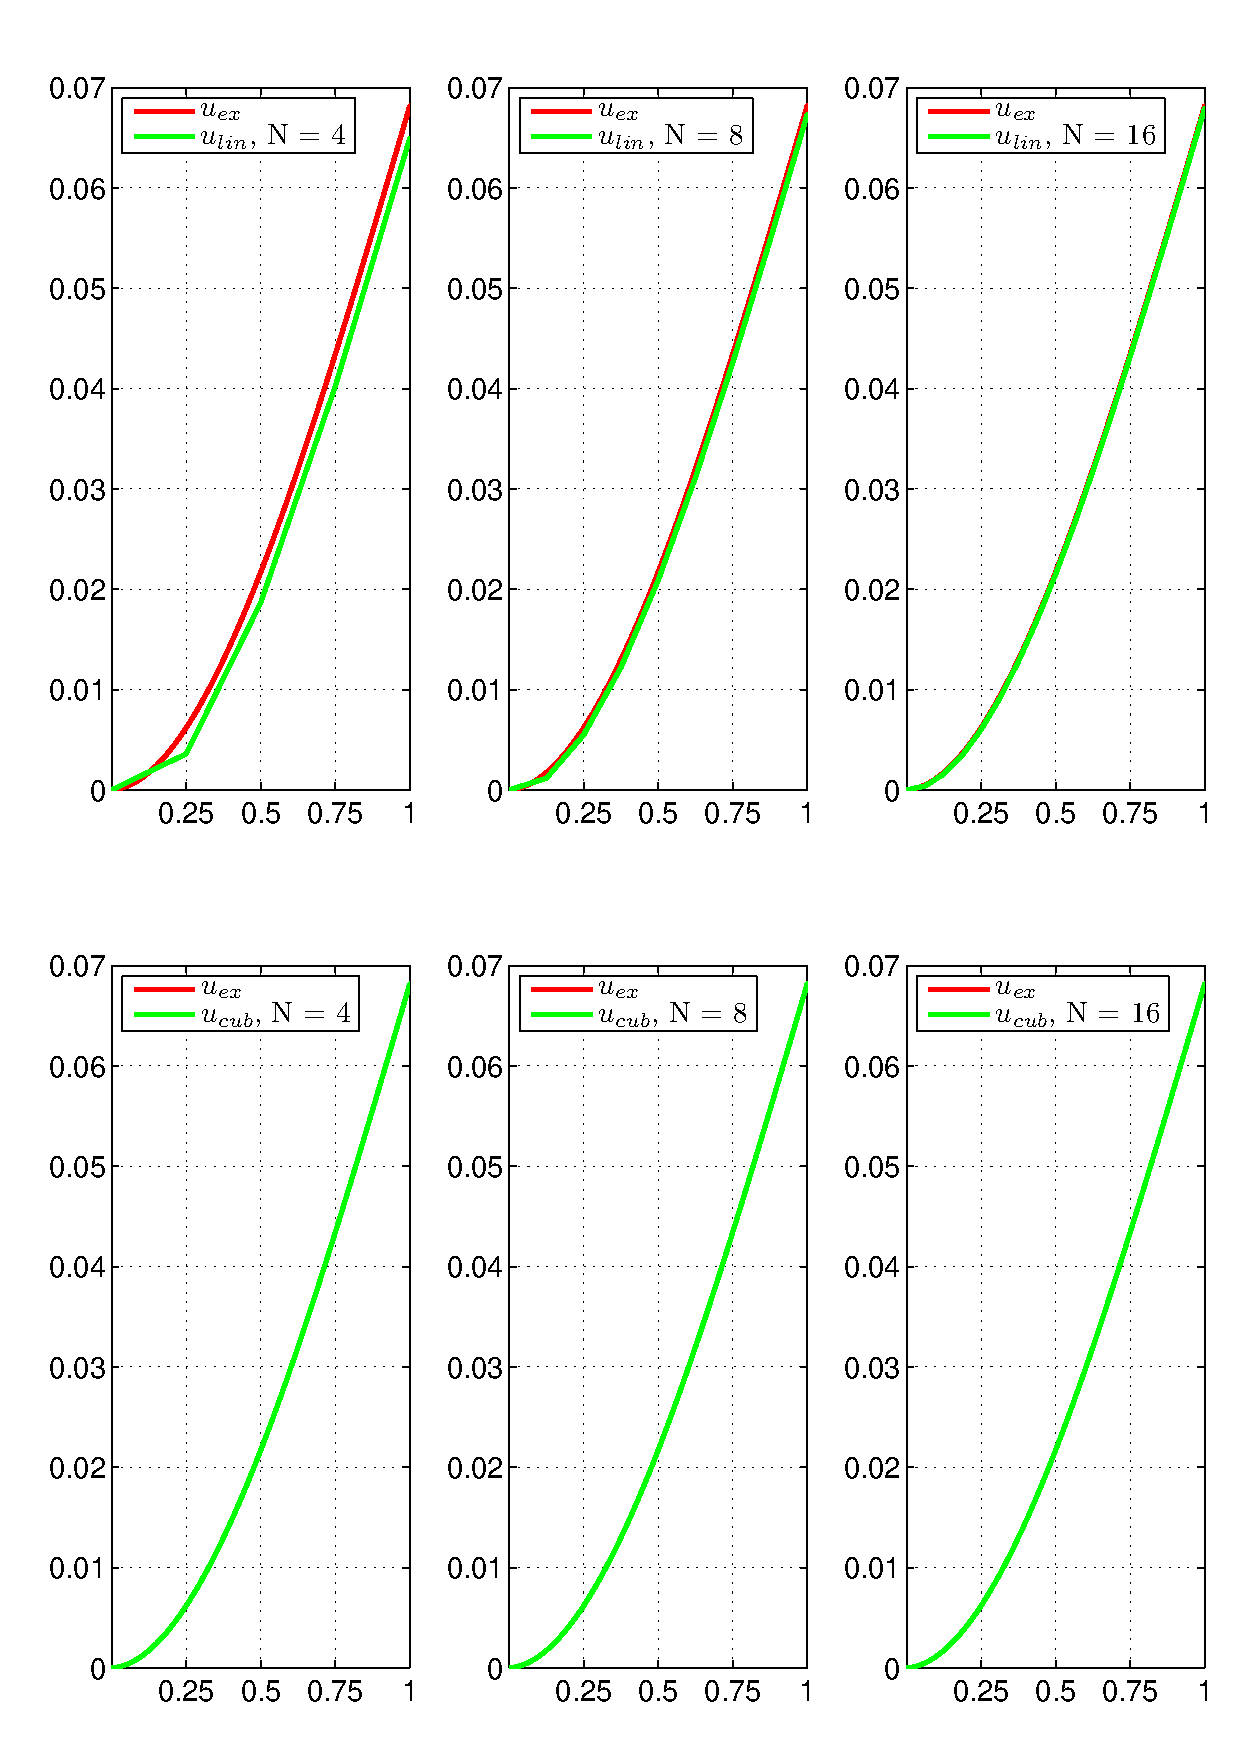
\includegraphics[width = \textwidth]{../figures/q-1-load-0}
	\caption[Analytical and \gls{FEMSol} of \cref{cas:q_1st_Degree_Denom} with a Uniform Load]
	{Analytical and \glspl{FEMSol} of \cref{cas:q_1st_Degree_Denom} with $e_1 = 10$ and $e_2 = 0.01$, a Uniform Load $\gls{f} = 1$
		and Boundary Parameters $\delta = 0$ and $P = 1$}
	\label{fig:q_1_Load_0}
\end{figure}
\begin{remark}
	As discussed in \cref{cha:Linear_Basis_Function}, \Glspl{linearFEMSol} support \glsentryname{order0Cont}. Thus
	the first derivative are discontinuous at \glspl{nodePoint}. This is clearly seen in node points when number of elements small,
	i.e., the upper left plots in \cref{fig:q_1_Load_0} The cubic solutions support, on the other hand, \glsentryname{order1Cont},
	see lower plots in the same figures.
\end{remark}
%

\section{Convergence Analysis}
To study convergence of a numerical solution we should define a measure for deviation between the analytical and numerical
approaches. In case of actual convergence we also need a factor that indicates speed of the process. Denote now
\begin{enumerate}
	\item \gls{u}: Exact solution of \cref{prb:Normalized_Problem}
	\item \gls{uNfem}: \Gls{FEMSol} of \cref{prb:Normalized_Problem} with $N$ elements. \\
				Note that $u_{N, \, fem}\left( x \right)$ might be
	\begin{itemize}
		\item \gls{uNlin}: Linear \gls{FEMSol} of \cref{prb:Normalized_Problem} with $N$ elements
		\item \gls{uNcub}: Cubic \gls{FEMSol} of \cref{prb:Normalized_Problem} with $N$ elements.
	\end{itemize}
\end{enumerate}
Define now following measures for solution deviations: \\
\begin{definition} \label{def:Squared_Error}
	In a Squared Error Measure we penalize the deviation between the numerical and analytical solutions by squaring its absolute
	value. Then we integrate this function over the whole region and take its square root, i.e.,
	\begin{equation}	\label{eqn:Squared_Error}
		\gls{ENsq} = \Bigg\{ \int_{x=0}^{1}\Big[ \gls{uEx} - \gls{uNfem} \Big] ^{2} \dd x \Bigg\}^{1/2}.
	\end{equation}
\end{definition}
%
\begin{definition}	\label{def:Max_Error}
	In a Max Error Measure we take absolute value of maximum deviation between the solutions, i.e.,
	\begin{align}	\label{eqn:Max_Error}
		\gls{ENmax} &= \max_{ 0 \leq x \leq 1 } \Big \vert  \gls{uEx} - \gls{uNfem} \Big \vert.
	\end{align}
\end{definition}
In this report we have chosen $E_{sq}$ for measuring the deviation. Having defined an error measure we move forward and define a
\gls{convFactor}.
%
\begin{definition} \label{def:Conv_Factor}
	Suppose that we have solved problem in \crefrange{eqn:FEM_Problem}{eqn:FEM_Right_Boundary} by applying \gls{FEM} with two different No.
	of elements, $N_{1}$ and $N_{2} = 2N_{1}$. Denote these solutions by $u_{1}$ and $u_{2}$ and let $E_{1}$
	and $E_{2}$ indicate the solution errors in the squared sense, see \cref{def:Squared_Error}. Define a \gls{convFactor} by
	\begin{equation} \label{eqn:Conv_Factor}
		\gls{fConv} = \frac{E_{1}}{E_{2}}.
	\end{equation}
\end{definition}
%
% Error estimates for the hyperbolic load
\begin{table}[tbh]
	\centering
	\rowcolors{1}{Gray}{LightCyan}
	\begin{tabular}{| c | c | c | c | c | c |} \hline
		% A constant
		\rowcolor{Cream} Load Function & $N$ & \gls{ENlin} & \gls{ENcub} & \gls{fConvLin} & \gls{fConvCub} \\ \hline
		$f_{n} \left( x \right) = 1$ & $4$ & \num{6.1 e-1} & \num{1.4 e-15} & - & -  \\ \hline
		$f_{n} \left( x \right) = 1$ & $8$	& \num{1.7 e-1} & \num{8.8 e-15} & $3.58$ & - \\ \hline
		$f_{n} \left( x \right) = 1$ & $16$ & \num{4.5 e-2} & \num{5.0 e-14} & $3.77$ & - \\ \hline
		% A linear function
		$f_{n} \left( x \right) = 1 + 2x$ & $4$	& \num{1.0 e0} & \num{5.6 e-4} & - & - \\ \hline
		$f_{n} \left( x \right) = 1 + 2x$ & $8$ & \num{2.8 e-1} & \num{3.4 e-5} & $3.61$&$16.3$ \\ \hline
		$f_{n} \left( x \right)=1 + 2x$ & $16$ & \num{7.3 e-2} & \num{2.1 e-6} & $3.79$ & $16.1$ \\ \hline
		% A quadratic function
		$f_{n} \left( x \right) = 1 + 2x - 3x^2$ & $4$ & \num{5.8 e-1} & \num{7.8 e-4} & - & - \\ \hline
		$f_{n} \left( x \right) = 1 + 2x - 3x^2$ & $8$ & \num{1.6 e-1} & \num{5.1 e-5} & $3.55$ & $15.3$ \\ \hline
		$f_{n} \left( x \right) = 1 + 2x - 3x^2$ & $16$	& \num{4.3 e-2} & \num{3.2 e-6} & $3.76$ & $15.8$ \\ \hline
	\end{tabular}
	\caption[Error Estimates for \glspl{FEMSol} of \cref{cas:q_1st_Degree_Denom}]
		{Error Estimates for \glspl{FEMSol} of \cref{cas:q_1st_Degree_Denom} with $e_1 = 10$ and $e_2 = 0.01$
		 and Boundary Parameters $\delta = 0$ and $P = 1$}
	\label{tbl:q_1st_Degree_Denom_Error}
\end{table}
%
% Error estimates for the classical problem with q(x) = e_1 / (x^2 + e_2)
\begin{table}
	\centering
	\rowcolors{1}{Gray}{LightCyan}
	\begin{tabular}{| c | c | c | c | c | c |} \hline
		\rowcolor{Cream} Load Function & $N$ & \gls{ENlin} & \gls{ENcub} & \gls{fConvLin} & \gls{fConvCub} \\ \hline
		% A constant
		$f_{n} \left( x \right) = 1$ & $4$ & \num{1.9 e-1} & \num{5.8 e-4} & - & - \\ \hline
		$f_{n} \left( x \right) = 1$ & $8$& \num{5.0 e-2} & \num{3.4 e-5} & $3.89$ & $17.0$	\\ \hline
		$f_{n} \left( x \right) = 1$ & $16$ & \num{1.3 e-2} & \num{2.1 e-6} & $3.94$ & $16.2$	\\ \hline
		% A linear function
		$f_{n} \left( x \right) = 1 + 2x$ & $4$	& \num{3.4 e-1} & \num{1.9 e-3} & - & - \\ \hline
		$f_{n} \left( x \right) = 1 + 2x$ & $8$	& \num{8.9 e-2} & \num{1.1 e-4} & $3.83$ & $16.7$ \\ \hline
		$f_{n} \left( x \right) = 1 + 2x$ & $16$ & \num{2.3 e-2} & \num{6.9 e-6} & $3.93$ & $16.2$ \\ \hline
		% A quadratic function
		$f_{n} \left( x \right) = 1 + 2x - 3x^2$ & $4$ & \num{1.7 e-1} & \num{8.6 e-4} & -& - \\ \hline
		$f_{n} \left( x \right) = 1 + 2x - 3x^2$ & $8$ & \num{4.2 e-2} & \num{6.2 e-5} & $3.94$ & $14.4$ \\ \hline
		$f_{n} \left( x \right) = 1 + 2x - 3x^2$ & $16$ & \num{1.1 e-2} & \num{4.0 e-6} & $3.95$ & $15.3$ \\ \hline
	\end{tabular}
	\caption[Error Estimates for \glspl{FEMSol} of \cref{cas:q_2nd_Degree_Denom}]
		{Error Estimates for \glspl{FEMSol} of \cref{cas:q_2nd_Degree_Denom} with $e_1 = 10$ and $e_2 = 0.01$ and Boundary Parameters $\delta = 0$ and $P = 1$}
	\label{tbl:q_2nd_Degree_Denom_Error}
\end{table}
%
% Error estimates for the exponential load
\begin{table}
	\centering
	\rowcolors{1}{Gray}{LightCyan}
	\begin{tabular}{| c | c | c | c | c | c |} \hline
		\rowcolor{Cream} Load Function & $N$ & \gls{ENlin} & \gls{ENcub} & \gls{fConvLin} & \gls{fConvCub} \\ \hline
		% A constant
		$f_{n} \left( x \right) = 1$ & $4$ & \num{1.3 e0}	& \num{4.2 e-3} & - & - \\ \hline
		$f_{n} \left( x \right) = 1$ & $8$	& \num{3.4 e-1} & \num{2.7 e-4} & $3.92$ & $15.6$ \\ \hline
		$f_{n} \left( x \right) = 1$ & $16$ & \num{8.5 e-2} & \num{1.7 e-5} & $3.98$ & $15.9$ \\ \hline
		% A linear function
		$f_{n} \left( x \right) = 1 + 2x$ & $4$	& \num{3.9 e0} & \num{1.9 e-2} & - & - \\ \hline
		$f_{n} \left( x \right) = 1 + 2x$ & $8$	& \num{1.0 e0} & \num{1.2 e-3} & $3.87$ & $15.5$ \\ \hline
		$f_{n} \left( x \right) = 1 + 2x$ & $16$ & \num{2.5 e-1} & \num{7.8 e-5} & $3.97$ & $15.9$ \\ \hline
		% A quadratic function
		$f_{n} \left( x \right) = 1+2x-3x^2$ & $4$ & \num{1.1 e0} & \num{1.7 e-2} & - & - \\ \hline
		$f_{n} \left( x \right) = 1+2x-3x^2$ & $8$ & \num{2.9 e-1} & \num{1.1 e-3} & $3.87$ & $15.0$ \\ \hline
		$f_{n} \left( x \right) = 1+2x-3x^2$ & $16$	& \num{7.4 e-2} & \num{7.0 e-5} & $3.96$ & $15.7$ \\ \hline

	\end{tabular}
	\caption[Error Estimates for \glspl{FEMSol} of \cref{cas:q_Exponential}]
		{Error Estimates for \glspl{FEMSol} of \cref{cas:q_Exponential} with $\alpha = 1$ and Boundary Parameters $\delta = 0$ and $P = 0.01$}
	\label{tbl:q_Exponential_Error}
\end{table}
Then the solution is convergent if $f_{con} > 1$ for all choices of $N_{1}$. Furthermore the larger $f_{con}$, the faster convergence. A value of $f_{c} = 4$, for example, indicates that doubling No. of elements results in a
reduction of the error by a factor $4$. Speed of convergence in this case is said to be of $\mathcal{O}\left( N^2\right) $. \\

Convergence speed of \glspl{FEMSol} in \cref{cas:q_1st_Degree_Denom,cas:q_2nd_Degree_Denom,cas:q_Exponential} is shown in \crefrange{tbl:q_1st_Degree_Denom_Error}{tbl:q_Exponential_Error}. A closer look at \cref{fig:q_1_Load_0} and \cref{tbl:q_1st_Degree_Denom_Error,tbl:q_2nd_Degree_Denom_Error} reveals the following facts:
\begin{enumerate}
	\item For a given \gls{N} it seems that both linear and cubic \glspl{FEMSol} stay on the same side of the \gls{analSol}, i.e., they do not oscillate around the \gls{analSol}.

	\item \Gls{linearFEMSol} seems to underestimate the displacement solution. \Gls{cubicFEMSol} on the other hand, changes between being larger and smaller than the \gls{analSol}.

	\item \Glsentryname{order0Cont} in \gls{linearFEMSol} is clearly seen when No. of elements is small, look at the \glspl{nodePoint} in upper left part of \cref{fig:q_1_Load_0}. Cubic \glspl{FEMSol} on the other hand,
	has continuous first derivative, see lower parts of \cref{fig:q_1_Load_0}.

	\item Obviously we can not satisfy the \gls{naturalCondition} with the \gls{linearFEMSol}, because it involves value of first derivative. In the cubic case, on the other hand, the solution has the exact derivative on the \gls{rightBoundary}.

	\item The linear and cubic \glspl{FEMSol} seem to converge as $\mathcal{O} \left( h^2 \right)$ and $\mathcal{O} \left( h^4 \right)$. This is in accordance with the results in \cref{cha:Error_Estimates}, see \cref{eqn:FEM_Error_To_h_And_Exact_Sol}.

	\item \Cref{fig:q_1_Load_0,tbl:q_1st_Degree_Denom_Error} suggest a cubic FEM-error comparable to the numerical round off error. This should not come as a surprise because the problem's \gls{analSol} is also a third degree polynomial, see \cref{eqn:q_1st_Degree_Denom_Solution}.

	\item Convergence speed decreases as by growing \gls{N}. This is of course due the round off error. This fact is more clear for cubic \gls{FEMSol} because of its faster speed of convergence.
\end{enumerate}	\text{}
%
Finally, the code in \cref{lst:Estimate_Error} estimates the squared error of \glspl{FEMSol} compared to the \gls{analSol} in each case.

